\chapter{Implementation}
\label{chapter:implementation}
This chapter will present the implementation of end-to-end network with its extensions.
First we start with docker to set the environment up. Next, we move onto LGSVL. Then, ROS.
From there a closed loop is achieved to collect data, preprocess, introduce neural
network, implement the models, and evaluate it. After achieving the basic results for the
preliminary architecture, sensor fusion techniques are implemented.

\section{Docker}
Docker is an open-source platform for developing, shipping and running applications.
Since, docker allows to setup the environment without knowing much about its internal
functionalities, we use docker for our implementation.

\subsection{Installation}

\begin{wrapfigure}{l}{0.5\textwidth}
	\centering
    \def\svgwidth{0.5\textwidth}
    \input{figures/inkscape/scrot_dockerengine.pdf_tex} %use full path to know the location of pdftex
    \caption{Docker Engine and its functions}
    \label{fig:dockerengine}
\end{wrapfigure}

A docker architecture, as shown in \ref{fig:dockerarchitecure}, consists of client, host
and registry. To make all these components work, docker daemon is necessary. A daemon is a
type of long-running background process. To get the daemon running, docker engine must be
installed first. After that, the LGSVL docker image is pulled from the registry using
\textit{docker pull} command. An image is a read-only template with instructions for
creating a docker container. The instructions are provided using a \textit{dockerfile}.
One can then build the images by themselves or use an image that is already built. In our
case since the image is readily available, so we use it.

A docker container for each task can be defined. Using along with a task, certain other
services may need to be run along with it. \textit{Docker compose} gives a perfect
solution to manage docker applications. A \textit{yaml} is configuration file which contains
definitions for the services. So we write script files for the services needed --
building the ros package, collecting data, and evaluating the trained model. For
services like preprocessing and training, docker is not used. Instead an anaconda
environment \cite{anacondaenv} is used because it reduces the hassles of installing tensorflow
 and its dependencies for training.

\section{LGSVL simulator}
The LGSVL simulator is developed using Unity engine which is written in C\# language.
The LGSVL team organises their code base\cite{lgsvlgithub} in such a way that makes it
easy for a beginner to learn the structure and implement new features or change the
existing ones.
\subsection{Web user interface and JSON sensor parameters}
The LGSVL team has developed a web UI to help users to configure maps, vehicles and
simulations. Different maps and vehicles can be downloaded from the LGSVL website. Even
customised maps and vehicles can be loaded to the simulator.
\iffalse
The figure
\ref{fig:lgsvlwebui} shows how the different tabs in web UI looks like.
\begin{figure}\centering
%\subfloat[Maps tab]
{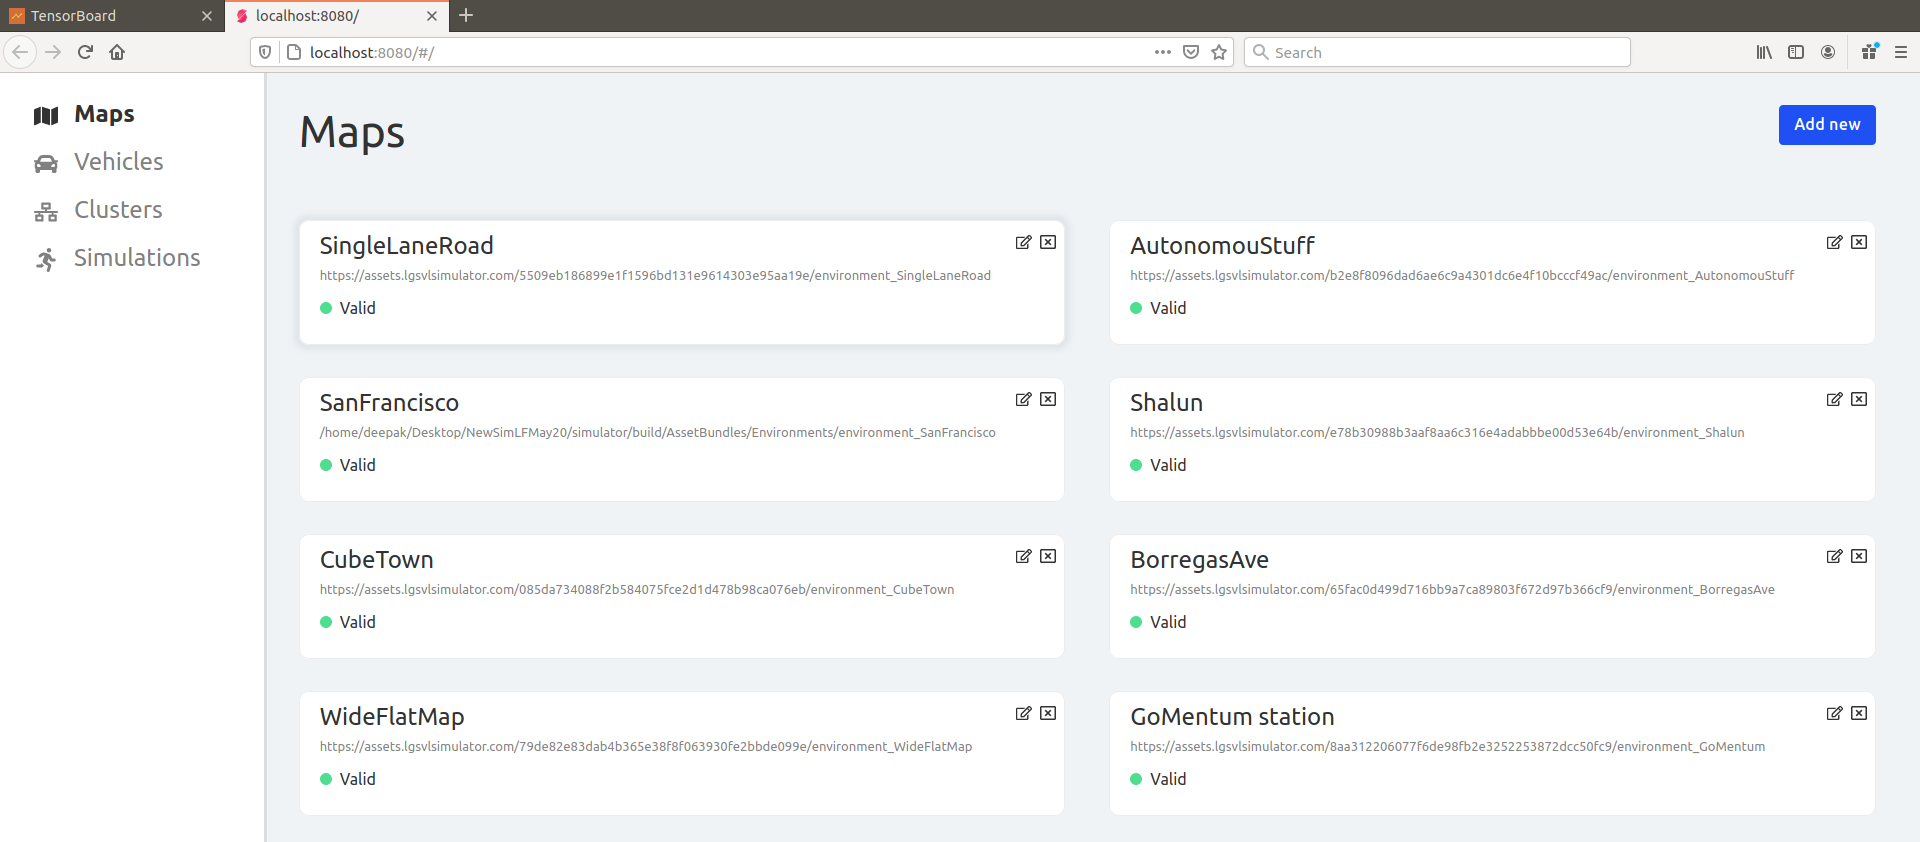
\includegraphics[scale=0.2]{figures/png/scrot_maps_tab.png}}
\par
%\subfloat[Vehicles tab]
{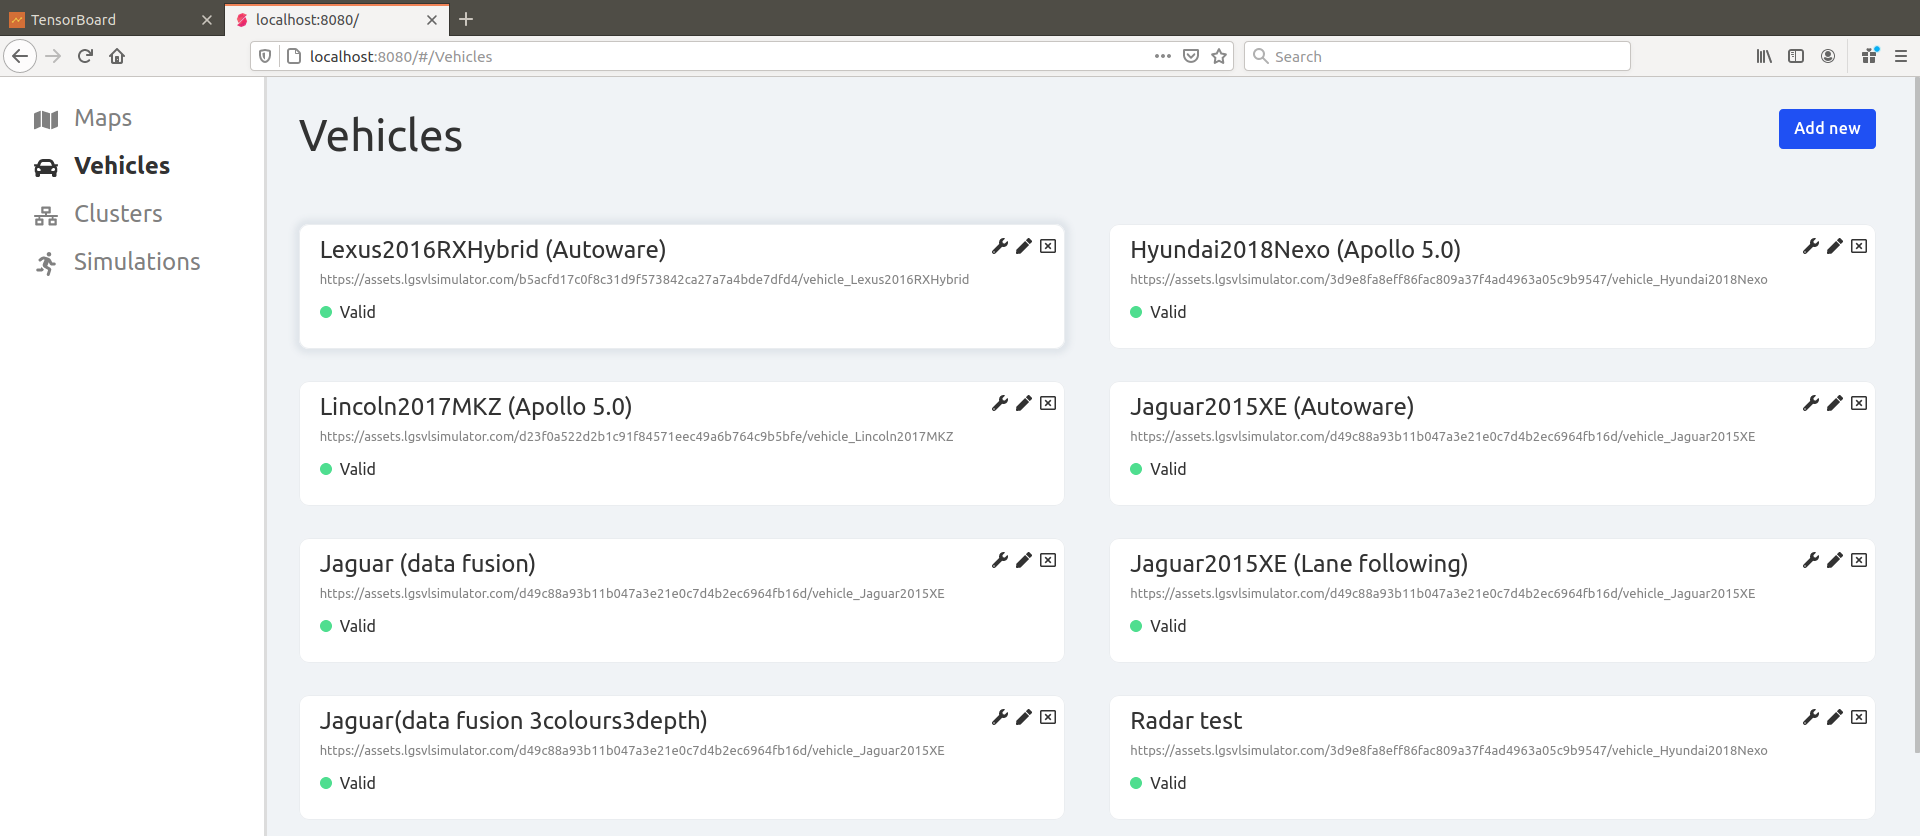
\includegraphics[scale=0.2]{figures/png/scrot_vehicles_tab.png}}
\par
%\subfloat[Simulations tab]
{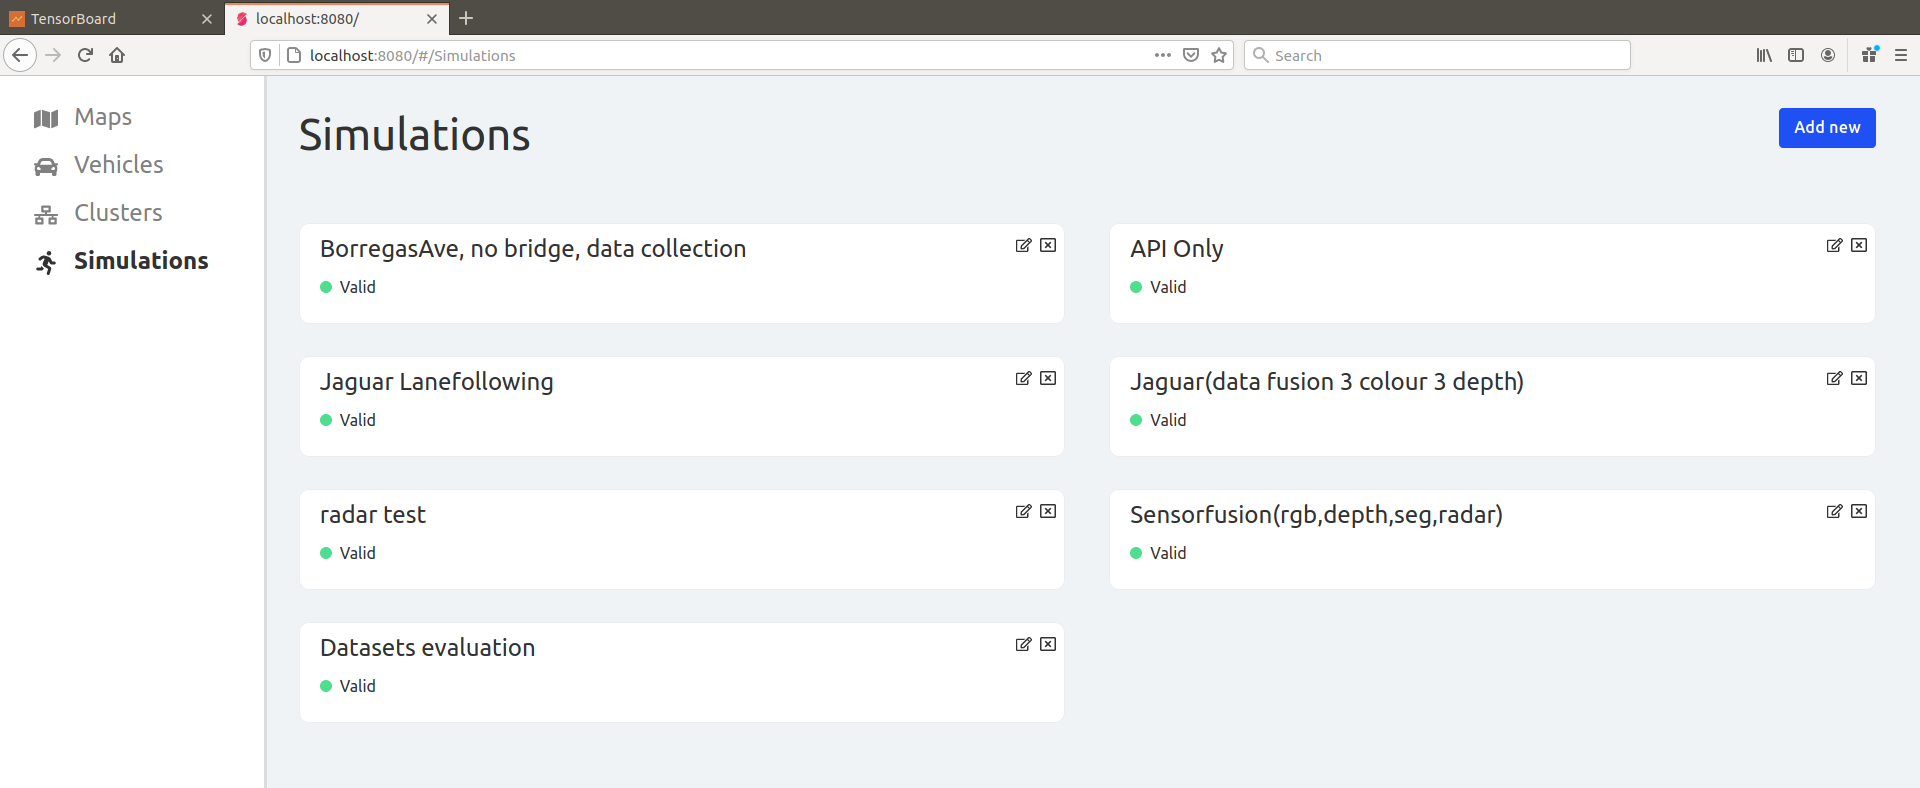
\includegraphics[scale=0.2]{figures/png/scrot_simulations_tab.png}
}
\caption{LGSVL Web UI}
\label{fig:lgsvlwebui}
\end{figure}
\fi
A sensor configuration is defined in JSON format. If a user wishes to use a colour camera
sensor then they need to use the JSON format appropriate for this sensor to the vehicle.
Each vehicle is provided with a configurable parameter field. The JSON has to be added
here. Each sensor has a topic name which is then used by ROS to subscribe to this topic.
There is also a space to define which bridge type to use for the particular sensor's
configuration.
\iffalse
\begin{lstlisting}
{
    "type": "Color Camera",
    "name": "Main Camera",
    "params": {
      "Width": 1920,
      "Height": 1080,
      "Frequency": 15,
      "JpegQuality": 75,
      "FieldOfView": 50,
      "MinDistance": 0.1,
      "MaxDistance": 2000,
      "Topic": "/simulator/main_camera",
      "Frame": "camera",
      "Distorted": true,
      "DistortionParameters": [
        -0.25349, 0.11868, 0, 0
      ]
    },
    "transform": {
      "x": 0,
      "y": 1.7,
      "z": -0.2,
      "pitch": 0,
      "yaw": 0,
      "roll": 0
    }
}

\end{lstlisting}
\fi
The file associated with each sensor then picks up these values and adjusts it in
run-time. If a sensor functionality is available, a user can use appropriate JSON to
utilise that sensor.
\subsection{Sensor plugin - Data collection and evaluation}
When a user doesn't want to disturb the current setup of the simulator but rather wants to add
some custom sensor to the vehicle configuration, then sensor plugin provides a perfect
solution. A set of guidelines must be followed while developing the plugin. In our case,
it is necessary to have a sensor plugin that would create a sensor and topics. This sensor
and these topics would then be used to fetch data from the simulator, transfer it through ROS bridge, and also receive
data for evaluation of the trained model. This custom plugin
extends the unity engine libraries to read the values from the JSON definition, fetch
values of steering, acceleration, braking from the vehicle control system, do
data transfer between simulator and ROS. The data transfer involves converting data types
to ROS understandable formats and convert back ROS to simulator formats during evaluation
phase.

\subsection{Radar Sensor}
Since data fusion is one of the goals of the thesis, using a radar sensor would provide
important depth information. However, in LGSVL, in its current version, the radar sensor is not working as
required. This necessitates some changes to some of the files in the LGSVL code base.
This process involves -
\begin{enumerate}
    \item Correcting the already existing radar sensor code to detect traffic properly and
        assign the data to their variables that look similar to ROS custom message standards.
    \item Convert the LGSVL data to ROS understandable  custom message formats.
    \item Add ROS2 as the bridge type to establish between client and LGSVL.
    \item On the client side, edit the docker to include custom radar message types.
\end{enumerate}

LGSVL simulator is now configured to send data towards the client. In order to reach the
client, as mentioned before, a ros bridge is needed. In the next section we will talk
about ROS and its uses.

\section{Data collection}
For data collection, \textit{python} programming language is used to create scripts. Each
script uses ROS components.

\subsection{ROS}
ROS, in our case, acts as an interface between simulator(server) and scripts(client).
We use ROS 2 and in particular \textit{dashing} iteration. The LGSVL follows the ROS standard for the message types.
The ROS nodes listen to the sensor topic(defined using JSON sensor parameter) and invoke
a callback whenever they receive data. Since each sensor receives at different rates, a
filter called message filters is used. With message filters, the queue size is set to a
higher value say 1000 and a delay(in seconds) through a \textit{slop} parameter of value
0.1 is used. This filter gathers all the subscribing nodes as one, synchronises
approximately to the delay parameter and invokes just one callback. This assures that data
from each listening node is present.

Inside the callback, the data is processed using computer vision(CV) and numpy libraries.
The ROS messages for the images include header and data
parts. The header part consists of the time at which the message is created and data part
contains the real data. With numpy libraries the real data is extracted easily for storage.

\subsection{ROS web bridge}
A ROS web bridge is virtual bridge between scripts using ROS and LGSVL simulator. In this
case, a ROS 2 web bridge, written in nodejs, is established. It basically starts an instance
that listens to an IP address and its port. The LGSVL on the other side, listens to this
IP address and port. Hence a bridge is created to allow flow of data.

\subsection{Building ROS2 package}
Before running the scripts with ROS, it must be built as ROS packages.  A package is a
container for ROS 2 code which makes it easier to share with others. Package creation in
ROS 2 uses \textit{ament} as its build system and \textit{colcon} as its build tool.
Packages can be created either in \textit{CMake} or \textit{Python}.

For CMake, \texttt{package.xml} and \texttt{CMakeLists.txt} files are necessary. \texttt{package.xml}
file contains meta information about the package. \texttt{CMakeLists.txt} file describes how to build the code within the package.

For Python, \texttt{setup.py}, \texttt{package.xml}, \texttt{setup.cfg} and
\texttt{resource/<package-name>} are needed. The \texttt{package.xml} file contains meta
information about the package. Unlike CMake, \texttt{setup.py} contains instructions for
how to install the package. The \texttt{setup.cfg} is required when a package has
executables, so \textit{ros2 run} can find them. Then finally \texttt{resource/<package-name>} a
directory with the same name as the package, used by ROS 2 tools to find the package,
contains \texttt{\twound{init}\twound{.py}}.

In our case, LGSVL team provides the base package. So we need to just build it using
\texttt{colcon build --symlink-install} command. But before building, the ROS2 environment
 must be set. It is important to remember that the package has
to be built every time a new ROS or custom message data types are introduced. A \texttt{build},
\texttt{install} and \texttt{log} directories are created along side \texttt{src}
directory when the build command is executed at the parent workspace directory. And
every time before running the package, its local environment must be set. Otherwise,
custom message data types won't be initialised.

\subsection{Using docker-compose services}
So everything that involves ROS starts with setting the environment globally or locally.
It is easy to miss this small step and encounter problems that could take a long time to
resolve. A \texttt{docker-compose} helps alleviate this problem. A service for each task
is implemented such as build, collect and evaluate. In the yaml file, each service has a
keyword to invoke the service and also an argument to link a file. In this case, a
shell script file is created. It contains all the necessary steps
such as setting the environment, starting the package, establishing ROS web bridge etc.

\section{Preprocessing}
The stored data can't be always used directly for training. Most times it must be
preprocessed to user's needs and goals.

Inputs are usually represented as X\_{data} and outputs as Y\_{data}. In our case, the input is images and output control commands.
Since we are doing supervised learning, we are aware about the outputs. These are stored in
\textit{csv} files along with file names of the images.

So, the first task in preprocessing is to select which Y\_data is necessary for prediction
and seperate them out into a small text file. Using this file, the images are fetched,
manipulated using CV2 libraries, stored in arrays and saved in the form of HDF5 files
\cite{hdf5file}. The Hierarchical Data Format version 5 (HDF5), is an open source file format
that supports large, complex, heterogeneous data. Within one HDF5 file, you can store a similar set of data organized in the same way that you might organize files and folders on your computer.
It is a compressed format and supports \textit{data slicing} which allows only a part of
the dataset to be read and not load all of them in the RAM memory.

The images in our case are read either as grayscale or RGB colour images. Then are cropped
and resized to a smaller resolution such as 160x70. For grayscale image there is one
channel. So the image's dimensions resemble 160x70x1 and for RGB image it has 3 channels
which means the dimensions are 160x70x3.

The images from multiple viewpoints or sensors can be fused together making
multi-channels. This task will be explained more in data fusion
section(\ref{sec:datafusion1}).

\subsection{LSTM}
LSTM comprises of serially lined up LSTM cells which allow prediction using previous
data. Since previous data require data from past, each frame image must be backtracked to
a certain, defined time period. This is called \textit{time steps}. According to the time
step, the images(frames) are gathered as one and stored. So for a $time\_step = 15$, the
dimensions will look like \texttt{15x70x160x1} for grayscale images and \texttt{15x70x160x3} for RGB
images.

\section{Datafusion}
\label{sec:datafusion1}
Data fusion is one of the primary goals of this thesis. As discussed in fundamentals
chapter(\ref{sec:datafusion}), there are two techniques for data fusion -- early and late
fusion. For early fusion, the images from multiple viewpoints or sensors are fused in the
preprocessing stage. This fusion is accomplished either by stacking the images or
concatenating them. So for example, if a grayscale and RGB images are fused/overlayed together using
concatenation, then the dimensions would like \texttt{70x160x4} where 4 represents number
of channels. These images are usually referred to as \textit{multispectral images}. The figure \ref{fig:cnnarchitecture} illustrates this approach.

Late fusion on the other hand is done during the training stage of the end-to-end work
flow. Usual process involves combining(concatenating) two sources of information after one
or two layers of convolution and then using the combined block to do further feature
extraction and eventually prediction. Or if the source is of a different modality than an
image, then it is unnecessary to fuse them in convolution stage. It is added after
the CNN is completed. However, it must be remembered that late fusion increases the
trainable parameters and costs on resources. The figure \ref{fig:latefusion} illustrates
one of the late fusion processes.

\begin{figure}[h]
    \centering
    \def\svgwidth{\textwidth}
    \input{figures/inkscape/latefusion1.pdf_tex}
    \caption{Late Fusion}
    \label{fig:latefusion}
\end{figure}

\section{Training the model}
Training a model involves designing a neural network architecture and deciding on its
hyperparameters. In this thesis, CNN and dense layers are designed with appropriate
activation functions, learning rate, epochs, batch size, CNN specific stride and kernel
lengths, optimizer etc.

\subsection{Loading from HDF5 and splitting the data}
The data stored in HDF5 files in preprocessing are loaded into memory as X\_data and
Y\_data respectively. Then using scikit-learn module, the X\_data is then split 80-20
as X\_train and X\_test respectively. And Y\_data as Y\_train and Y\_test respectively.

\subsection{CNN and fully connected layers}
For CNN layers, feature maps starting from 24 is chosen and gradually increased till 64.
The stride is always kept at 2 whereas the kernel size is (5,5) for the early and
(3,3) for the later stages. For early data fusion, the input is already with fused and directly
fed to the neural network. However, for late fusion, concatenation is done at appropriate
stages. If necessary, max pooling and batch normalization layers are added to the neural
network. Most often to distribute the features uniformly and make the cost function
distribute symmetrically, the inputs are normalized. In this case, since images are pixel
values between 0-255, each pixel is divided by 255 to bring it in the range between 0 and
1.

Since Keras is used, almost all the layers can be implemented in a fewer lines of code.
Activation functions are given as an argument to a layer. Adding new layers is easier with
functional API \ref{subsec:modelsapi}. When the convolutional layers' output needs to be
flattened to form a vector, \texttt{Flatten} command is called.

The fully connected or dense layers take input as a vector. The hyperparameters are
adjusted accordingly to avoid overfitting. Using dropout layers and batch normalization
help alleviate this problem.

Using callbacks functionality of Keras, the best model is saved in HDF5 file. In our case, validation
loss  reaching the minimum is monitored. Since the datasets are not huge, an epoch of 100
is sufficient.

\section{Evaluation}
The trained model is saved as HDF5 file format. Evaluation is basically completes the loop
of end-to-end training architecture. The trained model is placed at a location the
evaluation script can access. Then from the LGSVL simulator data are received through ROS
bridge and subscriber nodes. With the help of message filters, the messages are collected.
Inside the callback, the image manipulation carried out in preprocessing phase, is
repeated. The preprocessed image is then fed to the trained model. The models predicts the
output. In our case, control commands. These commands are then assigned and published/sent
back to the simulator through ROS bridge. The custom plugin has a subscribing topic on the
LGSVL side. The data sent through ROS bridge, is listened in this topic. The predicted command behaviour is observed and
evaluated using appropriate metrics. It is important to remember the exact steps followed
in preprocessing must be repeated while evaluated. Otherwise, it will lead to inconsistent
performance.
\iffalse
\section{What to include here?}

\begin{enumerate}
    \item Docker - Dockerfile contents - docker scripts - how they are invoked.
    \item LGSVL - C\# language, Unity engine, code organisation, sensor plugin and its
        structure, data type conversion, WebUI - JSON- sensors used. Making Radar work,
        Increasing traffic density and time at the signal.
    \item Data collection - ROS2- ros2 message types - topics - msgfilters -
        approx-sync - callback- cv2 libraries - saving. Also ROS2 web bridge.
    \item Preprocessing - CV2 image manipulation - stacking, concatenate  -
        Time series LSTM stuff - saving in HDF5.
    \item Training - Loading hdf5 - splitting data - Functional API - normalisation
        - datafusion - early, late - concat - batch normalisation - stride - kernel -
        flatten - FC - prediction - Activation function - loss function - learning rate -
        optimizer - epochs - shuffling - batch size - callbacks - ES - MC - TB - saving
        models.
    \item Evaluation - similar stuff to data collect - image manipulation - prediction -
        publishing. How to validate evaluation?

\end{enumerate}

\fi
